% adapté de la RIG version française

\documentclass[french]{./sageo}

\confShortName{SAGEO'2017}
\confLongName{SAGEO'2017 - Rouen, 6-9 novembre 2017}

\usepackage[utf8]{inputenc} 
\usepackage[T1]{fontenc}
\usepackage{lmodern}
\usepackage{textcomp}
\usepackage{amsmath}
\usepackage{graphicx}
\usepackage{multirow}
\usepackage[noend]{algorithmic}
\usepackage[linesnumbered,ruled,vlined,boxed,commentsnumbered]{algorithm2e}

\firstpagenumber{1}

% \title[short header title]{title}
\title[Causalités Spatio-temporelles]{Une méthode d'identification de causalités dans des données spatio-temporelles}

\author[1,2]{Juste}{Raimbault}


% addresses are automatically numbered
\address{UMR CNRS 8504 Géographie-cités}
        {}
\address{UMR-T 9403 IFSTTAR LVMT}
        {juste.raimbault@polytechnique.edu}       

\resume{Résumé.}


\motscles{Quelques mots clés}

\keywords{En anglais}

\abstract{Abstract in English}

\begin{document}

\maketitle

\newpage



%%%%%%%%%%%%%%%
\section{Introduction}
%%%%%%%%%%%%%%%



L'étude des processus spatio-temporels fortement couplés implique des relations entre processus complexes à isoler. Les régimes sous lesquels des identifications de causalité sont cohérentes ne sont pas non plus identifiés de manière évidente. La définition de la causalité


\cite{liu2011discovering} propose la detection de relations spatio-temporelles entre perturbations des flots de trafic, introduisant une définition particulière de la causalité basé sur une correspondance de points extrêmes. Les algorithmes associés sont toutefois spécifiques et difficilement applicables à des types de systèmes différents.

Les neurosciences ont développé de nombreuses méthodes répondant à des problématiques similaires. \cite{luo2013spatio} définit une causalité de Granger généralisée prenant en compte la non-stationnarité et s'appliquant à des régions abstraites issues d'imagerie fonctionnelle.



%%%%%%%%%%%%%%%
\section{Méthode}
%%%%%%%%%%%%%%%


Nous décrivons ici une méthode générique, basée sur un test similaire à la causalité de Granger~\cite{}, pour tenter d'identifier des relations causales dans des systèmes spatiaux. Soit $X_j(\vec{x},t)$ des processus aléatoires spatiaux unidimensionnels. Une réalisation d'un sous-système territorial est donnée par des ensembles de trajectoires pour chaque processus $x_{i,j,t}$. On suppose l'existence de fonctions de correspondance $\Phi_{j1,j2}$ permettant de faire correspondre les réalisations de chaque composantes à un index unique (dans le cas le plus simple, on associera les variables sur les mêmes patches). Si $\textrm{argmax}_{\tau} \hat{\rho}\left[x_{j_1},x_{j_2}\right]$ est clairement défini % TODO notion trop floue ? le problème est que des modèles stat conditionnent trop ?
, son signe donnera alors le sens de la causalité entre les composantes $j_1$ et $j_2$.


% TODO some kind of smoothing has to be introduced, either as preprocessing or as part of the optimization process (at least for first observed behavior on synthetic data. maybe it is typical of the model ?)
% - formalize mean estimator on repetitions, compare it to a direct estimator (// computation or aggregated data ?)







%%%%%%%%%%%%%%%
\section{Résultats}
%%%%%%%%%%%%%%%


%%%%%%%%%%%%%%%
\subsection{Données Synthétiques}

Cette méthode doit dans un premier temps être testée et partiellement validée, ce que nous proposons de faire sur des données synthétiques. % cit Rochebrune ?
 \cite{raimbault2014hybrid} est un modèle simple de morphogenèse urbaine (modèle RBD) faisant un candidat intéressant pour notre test. En effet, les variables explicatives de la croissance urbaine, les processus d'extension du réseau et le couplage entre densité urbaine et réseau sont assez élémentaires. Cependant, hormis dans des cas extrêmes (distance au centre détermine valeur foncière uniquement, le réseau dépendra de manière causale de la densité, ou distance au réseau seule, la causalité devrait être inversée), les régimes mixtes n'exhibent pas de causalités évidentes : c'est donc un parfait cas pour tester si la méthode est capable d'en détecter.

Nous explorons une grille de l'espace des paramètres du modèle RBD. Pour chaque valeur des paramètres, nous procédons à $N=100$ répétitions. % Le modèle a par ailleurs été exploré de nouveau pour reproduction et extension des résultats. % TODO appendice with full RBD exploration.
Nous calculons sur l'ensemble des patches les corrélations retardées entre les variables suivantes : densité locale, distance au centre et distance au réseau. Une grille de pas 0.5 (26 combinaisons) est entièrement explorée en Appendice~\ref{}. Des regroupements par régimes peuvent se faire, lorsqu'un paramètre domine et impose le régime (par exemple )







%%%%%%%%%%%%%%%
\subsection{Cas d'étude}




%%%%%%%%%%%%%%%
\section{Discussion}
%%%%%%%%%%%%%%%




%%%%%%%%%%%%%%%
\section{Conclusion}
%%%%%%%%%%%%%%%





%%%%%%%%%%%%%%%
%% Biblio
%%%%%%%%%%%%%%%

\bibliography{biblio,/Users/Juste/Documents/ComplexSystems/CityNetwork/Biblio/BibTeX/CityNetwork}







%%%%%%%%%%%%%%%
%% TEMPLATES
%%%%%%%%%%%%%%%

%
%
%
%\section{Section 1}
%
%\subsection{Sous-section 1}
%
%\subsubsection{Sous-sous-section 1}
%
%\begin{figure*}[h]
%   \centering  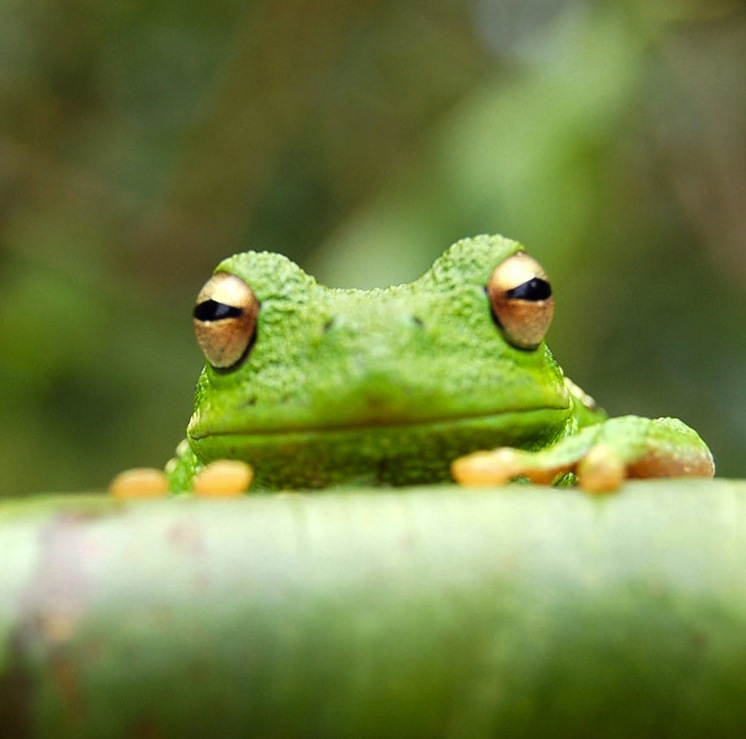
\includegraphics[width=8cm]{grenouille.jpg}
%  \caption{\label{fig:1} Une grenouille bien verte.}
%\end{figure*}
%
%\subsection{Sous-section 2}
%
%\section{Section 2}
%
%Listes :
%\begin{itemize}
%\item ligne 1 (cf. équation \ref{eq:form1})
%\item ligne 2 (cf. équation \ref{eq:form2})
%\end{itemize}
%
%Formules :
%
%\begin{equation}
%	R = \frac{d_1}{d_2}
%	\label{eq:form1}
%\end{equation}
%
%\begin{equation}
%	\sin(\alpha) = \frac{h}{l}
%    \label{eq:form2}
%\end{equation}
%
%\begin{table*}[h!]
%\begin{center}
%\caption{\label{tab:1} Exemple de tableau}
% \scriptsize
%      \begin{tabular}{|c|c|c|c|c|}
%   \hline
%   \multirow{2}*{ Clients} & \multicolumn{2}{| c |}{Départ }  & \multicolumn{2}{| c |}{ Arrivée}\\
%   \cline{2-5}
%      & Station  & Période de Temps & Station  & Période de Temps \\\hline
%   client 1 (c1) & 3  & 2 & 1 & 4 \\\hline
%   client 2 (c2)   &   2  & 2 & 3 & 3\\\hline
%   client 3 (c3)   &   2 & 2 & 3 & 4  \\\hline
%   client 4 (c4)   &   3 & 2 & 2 & 3  \\\hline
%   client 5 (c5)   &   3 & 2 & 2 & 4  \\\hline
%  client 6 (c6)   &   2  & 4 & 3 & 5\\\hline
%   client 7 (c7)   &   3  & 3 & 2 & 6  \\\hline
%   client 8 (c8)   &   1 & 5 & 3 & 6 \\\hline
%   client 9 (c9) & 2  & 6 & 3 & 7 \\\hline
%    client 10 (c10)  &   3 & 7 & 1 & 9 \\\hline
%   client 11 (c11) & 1  & 6 & 2 & 7 \\\hline
%%\hline
%\end{tabular}
%\end{center}
%\end{table*}
%
%Exemple d'algorithme :
%
%\begin{algorithm}[h!]
%\label {algo}
% \KwData{
% $G(V,A,C,R,U)$ \; \tcc{commentaire}}
% \KwResult{
% $Paths_{Cars}, \; Relocation,\; SatisfiedDemands, Paths_{Agents}  $
% }
% initialization\;
% $Paths_{Agents} \gets \emptyset $ /* l'ensemble de chemins... */ \;
% $j \gets 1$ \;
% $costPath_j  \gets 0$ \;
% \While { $ (j \le  nb_{Veh}) \wedge (costPath_j \leq 0)  $ }
% {
% $ path_j \gets Dijkstra(G(V,A, C,R)) $ \;
%$ costPath_j \gets  Cost (path_j)$ \;
%  \ForAll { $(v^{k}_{t'},v^{i}_{t}) \in path   $}
%{
% \ForAll {$ U_{r^{i}_{t'',t''+1}} $  }
% {....
% }
%$ Paths_{Cars} \gets Paths_{Cars} \cup path_j $  \;
% }
%$j \gets j+1$ \;
% }
%$Paths_{Agents} \gets  routeAgents (Relocation ); $
% \caption{un algorithme très glouton}
%\end{algorithm}
%









\end{document}